\documentclass{article}
\usepackage[utf8]{inputenc}
\usepackage[T1]{fontenc}
\usepackage[utf8]{inputenc}
\usepackage{amsmath}
\usepackage{tikz,pgfplots}
\usepackage{tikz-network}
\usetikzlibrary{shapes,decorations,arrows,calc,arrows.meta,fit,positioning}
\usepackage{color, colortbl}

\begin{document}

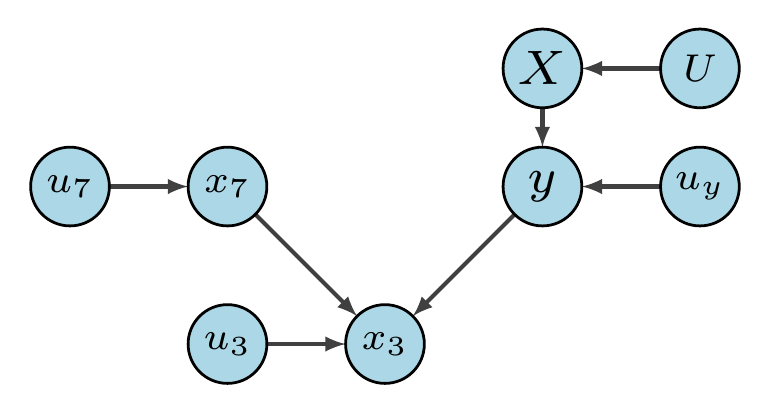
\begin{tikzpicture}
\Vertex[x=1,size = 1,y=-2,label = $u_3$, fontscale = 2]{u3}
\Vertex[x=1,size = 1,label = $x_7$, fontscale = 2]{x7}
\Vertex[size =1, x=5,label = $y$, fontscale =2.5]{Y}
\Vertex[size =1, x=5,y=1.5,label = $X$, fontscale =2.5]{X}
\Vertex[size=1,x=3,y=-2,fontscale = 2,label = $x_3$]{x3}
\Vertex[size=1,x=7,label = $u_y$,fontscale = 2]{Uy}
\Vertex[size=1,x=-1,label = $u_7$,fontscale = 2]{U7}
\Vertex[size=1,x=7,y = 1.5,label = $U$,fontscale = 2]{U}
\Edge[Direct](Uy)(Y)
\Edge[Direct](X)(Y)
\Edge[Direct](U)(X)
\Edge[Direct](u3)(x3)
\Edge[Direct](U7)(x7)
\Edge[Direct](x7)(x3)
\Edge[Direct](Y)(x3)
\end{tikzpicture}

\end{document}